\section{Introduction}

We start with two random variables $X_1$ and $X_2$ jointly distributed with probability density function $f(X_1, X_2)$, that is,

\begin{align*}
(X_1, X_2) \sim f(x_1, x_2)
\end{align*}

We also have marginal densities,

\begin{align*}
f_{X_1}(x_1) &= \int_{\mathbb{R}}f(x_1, x_2)\, \mathrm{d}x_2\\ 
f_{X_2}(x_2) &= \int_{\mathbb{R}}f(x_1, x_2)\, \mathrm{d}x_1\\ 
\end{align*}

Recall that $X_1 \perp X_2$ iff $f(x_1, x_2) = f_{X_1}(x_1)f_{X_2}(x_2)$. The cumulative probability density of each $X_1$ and $X_2$ are,

\begin{align*}
F_{X_1}(x_1) &= \int_{-\infty}^{x_1}f_{X_1}(t)\,\mathrm{d}t\\
F_{X_2}(x_2) &= \int_{-\infty}^{x_2}f_{X_2}(t)\,\mathrm{d}t
\end{align*}

Finally we have the polymorphic expectation operator,

\begin{align*}
\mathbb{E}[X_1] &= \int_{\mathbb{R}} x_1 f_{X_1}(x_1)\,\mathrm{d}x_1\\
\mathbb{E}[X_1] &= \int_{\mathbb{R}^2} x_1 f(x_1,x_2)\,\mathrm{d}x_1\mathrm{d}x_2\\
\mathbb{E}[u(X_1, X_2)] &= \int_{\mathbb{R}^2} u(x_1, x_2) f(x_1,x_2)\,\mathrm{d}x_1\mathrm{d}x_2
\end{align*}

where the last line is the required form is $u()$ is non-trivially a function of both $x_1$ and $x_2$. We then see variance as a special case of $\mathbb{E}[u(x_1, x_2)]$,

\begin{align*}
Var(X_2) &= \mathbb{E}[(X_2 - \mathbb{E}[X_2])^2]\\
         &= \mathbb{E}[X_2^2] - \mathbb{E}[X_2]^2
\end{align*}

also known as the second central moment. There are other moments, but we don't care at this point.

A physical analog may be see with probability density equated with mass density and random variables such as $X_1$ and $X_2$ as distance. Then $\mathbb{E}[X_2]$ is the center of mass of a 2D distribution of mass about a point along the $X_2$ axis. Similarly $Var(X_2)$ is the moment of intertia about the center (line) of mass $\mathbb{E}[X_2]$.

If we peek ahead at \ref{fig:ConditionalExpectation} we see a triangular indicating the set of non-zero probability density. The horizontal line market $\mathbb{E}[X_2]$ is the center of mass along the $X_2$ axis about which a physical triangle may spin (out of the page).

\section{Conditional Probability}

Suppose that $A$ and $B$ are two events. The definition of conditional probability is,

\begin{align*}
P(B | A) = \frac{P(A \cap B)}{P(A)} \; \text{ if $P(A) \ne 0$}
\end{align*}

This conditional definition may be avoided if we recognize that $A | B$ implies that $B \in \Omega$ is now the whole space so that $P(B | B) \equiv 1$. Then we write the unconditional statement,

\begin{align*}
P(A \cap B) = P(B | A) P(A)
\end{align*} 

which carries it's own insight, which is that joint events may be computed sequentially. This particular insight will be used to decomponse the joint density functions and associated expectations into manageable fragments.

\begin{figure}
  \centering
  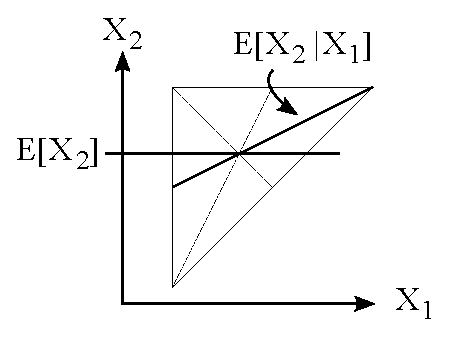
\includegraphics{Images/ConditionalExpectation.eps}
  \caption[Mean and Conditional Mean]
          {Mean and Conditional Mean}
  \label{fig:ConditionalExpectation}
\end{figure}

The probability density analog of the conditional probability statement is,

\begin{align*}
f_{X_2 | X_1 = x_1}(x_2) = \frac{f(x_1, x_2)}{f_{X_1}(x_1)}
\end{align*}

taking careful note of the upper-case (random variable) and lower-case (particular value). At this point we introduce some notational convenience,

\begin{align*}
f_1 &\equiv f_{X_1}\\
f_{2|1} &\equiv f_{X_2 | X_1 = x_1}
\end{align*}

To check that the conditional density function is valid we integrate it,

\begin{align*}
\int_{-\infty}^\infty f_{X_2 | X_1 = x_1}(x_2) \,\mathrm{d}x_2
&= \int_{-\infty}^\infty \frac{f(x_1, x_2)}{f_{X_1}(x_1)} \,\mathrm{d}x_2\\
&= \frac{1}{f_{X_1}(x_1)}\int_\mathbb{R} f(x_1, x_2) \,\mathrm{d}x_2\\
&= \frac{1}{f_{X_1}(x_1)}f_{X_1}(x_1)\\
&= 1
\end{align*}

Now we can define conditional expectation,

\begin{align*}
\mathbb{E} \left[X_2 | X_1 \right] 
&= \int_{-\infty}^\infty x_2 \, f_{X_2 | X_1}(x_2) \,\mathrm{d}x_2\\
&= \int_{-\infty}^\infty x_2 \, f_{2|1}(x_2) \,\mathrm{d}x_2 \in X_1
\end{align*}

where we emphasize that the result is a function of $X_1$. Recall that $\mathbb{E}[]$ is polymorphic and therefore it's meaning depends on context. The following should now be clear,

\begin{align}
\mathbb{E}\left[\mathbb{E}\left[X_2 | X_1 \right] \right]
&= \int_{-\infty}^\infty\int_{-\infty}^\infty x_2 \, f_{2|1}(x_2)\,\mathrm{d}x_2 f_1(x_1) \,\mathrm{d}x_1\\
&= \int_{-\infty}^\infty\int_{-\infty}^\infty x_2 \, f(x_1, x_2)\,\mathrm{d}x_2\mathrm{d}x_1\\
\label{eq:exp_exp} &= \mathbb{E}\left[X_2\right]
\end{align}

The figure \ref{fig:ConditionalExpectation} shows both the constant $\mathbb{E}[X_2]$ and the function of $X_1$, namely $\mathbb{E}[X_2 | X_1]$. Recall that the line $\mathbb{E}[X_2 | X_1]$ may not appear to resolve to $\mathbb{E}[X_1]$ on average, but it is a weighted average with, in the case of the figure, more weight associated with the left-most values of the line and less to the right-most values.

Now consider the conditional variance as it relates to unconditional variance. We start with the basics,

\begin{align}
\label{eq:var}      Var(X_2)       &= \mathbb{E}[X_2^2] - \mathbb{E}[X_2]^2\\
\label{eq:cond_var} Var(X_2 | X_1) &=  \mathbb{E}[X_2^2 | X_1] - \mathbb{E}[X_2 | X_1]^2
\end{align}

Now we do two things. We take the expectation of \ref{eq:cond_var},

\begin{align}
\mathbb{E}[Var(X_2 | X_1)] 
&= \mathbb{E}[\mathbb{E}[X_2^2 | X_1]] - \mathbb{E}[\mathbb{E}[X_2 | X_1]^2]\\
\label{eq:exp_cond} &= \mathbb{E}[X_2^2] - \mathbb{E}[\mathbb{E}[X_2 | X_1]^2]
\end{align}

then we find the variance of the conditional expectation,

\begin{align}
Var(\mathbb{E}[X_2 | X_1]) 
&= \mathbb{E}[\mathbb{E}[X_2 | X_1]^2] - \mathbb{E}[\mathbb{E}[X_2 | X_1]]\\
\label{eq:var_cond} &= \mathbb{E}[\mathbb{E}[X_2 | X_1]^2] - \mathbb{E}[X_2]^2
\end{align}

Noting that \ref{eq:var} =  \ref{eq:exp_cond} + \ref{eq:var_cond} we find our main result,

\begin{align}
\boxed{
Var(X_2) = \mathbb{E}[Var(X_2 | X_1)] + Var(\mathbb{E}[X_2 | X_1])
}
\end{align}

Our take-away is that, on average, the variance of a conditioned variable tends to be less that the variance of that same variable, unconditioned. Referring to figure \ref{fig:ConditionalExpectation} our physical analog is that the rotational inertia of the triangle is less than the $\mathbb{E}[X_2 | X_1]$ line. The difference is the average rotational inertia along the $\mathbb{E}[X_2 | X_1]$ line.
